\section{Method}
\ref{sec:method}


\subsection{Power supply (PSU)}
The subsystems require 5V respective 3.3V. With all subsystem powered on it draws around 1A.
Power supply consist of LT1086 voltage regulator which is capable of delivering 1.5A.
Two PSU was made to supply 5V respective 3.3V.
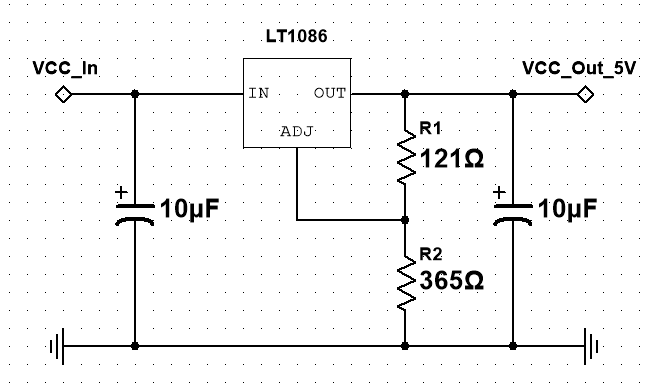
\includegraphics[width=\linewidth]{voltage_regulator}



\subsection{UART}
For sensors which is communicating between 3.3V and 5V TTL over UART is using a voltage divider to interface.
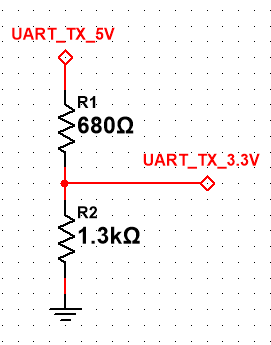
\includegraphics[width=\linewidth]{voltage_divider}




\subsection{Packet}
Communication between Arduino, ESP8266, NodeJS server is done via custom packet of 12 Bytes data.
Packet consist of 2 bytes start flags, 1 bytes checksum, 1 bytes data kind, 4 bytes data value, 4 bytes timestamp.

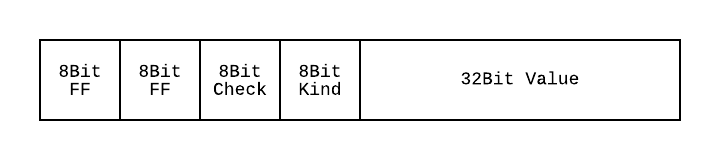
\includegraphics[width=\linewidth]{packet1}


\subsection{Sensor MQ-4}
Measures LPG, Methane (CH4), H2, CO, Alcohol, Smoke.
Sensor is composed by micro AL2O3 ceramic tube, Tin Dioxide (SnO2) sensitive layer,
measuring electrode and heater are fixed into a crust made by plastic and stainless steel net.

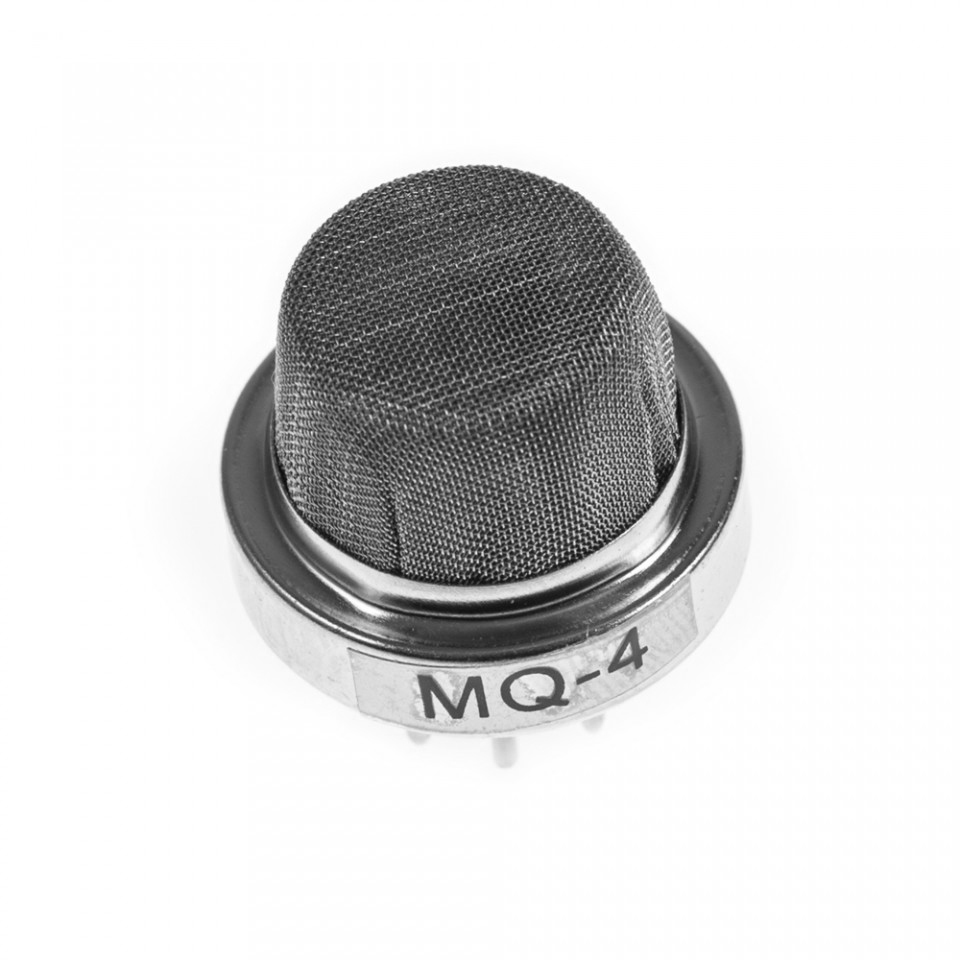
\includegraphics[width=0.5\linewidth]{MQ4}

\subsection{Sensor MQ-2}
Measures LPG, Methane (CH4), H2., CO, Alcohol, Propane, Smoke.
Sensor is composed by micro AL2O3 ceramic tube, Tin Dioxide (SnO2) sensitive layer,
measuring electrode and heater are fixed into a crust made by plastic and stainless steel net.

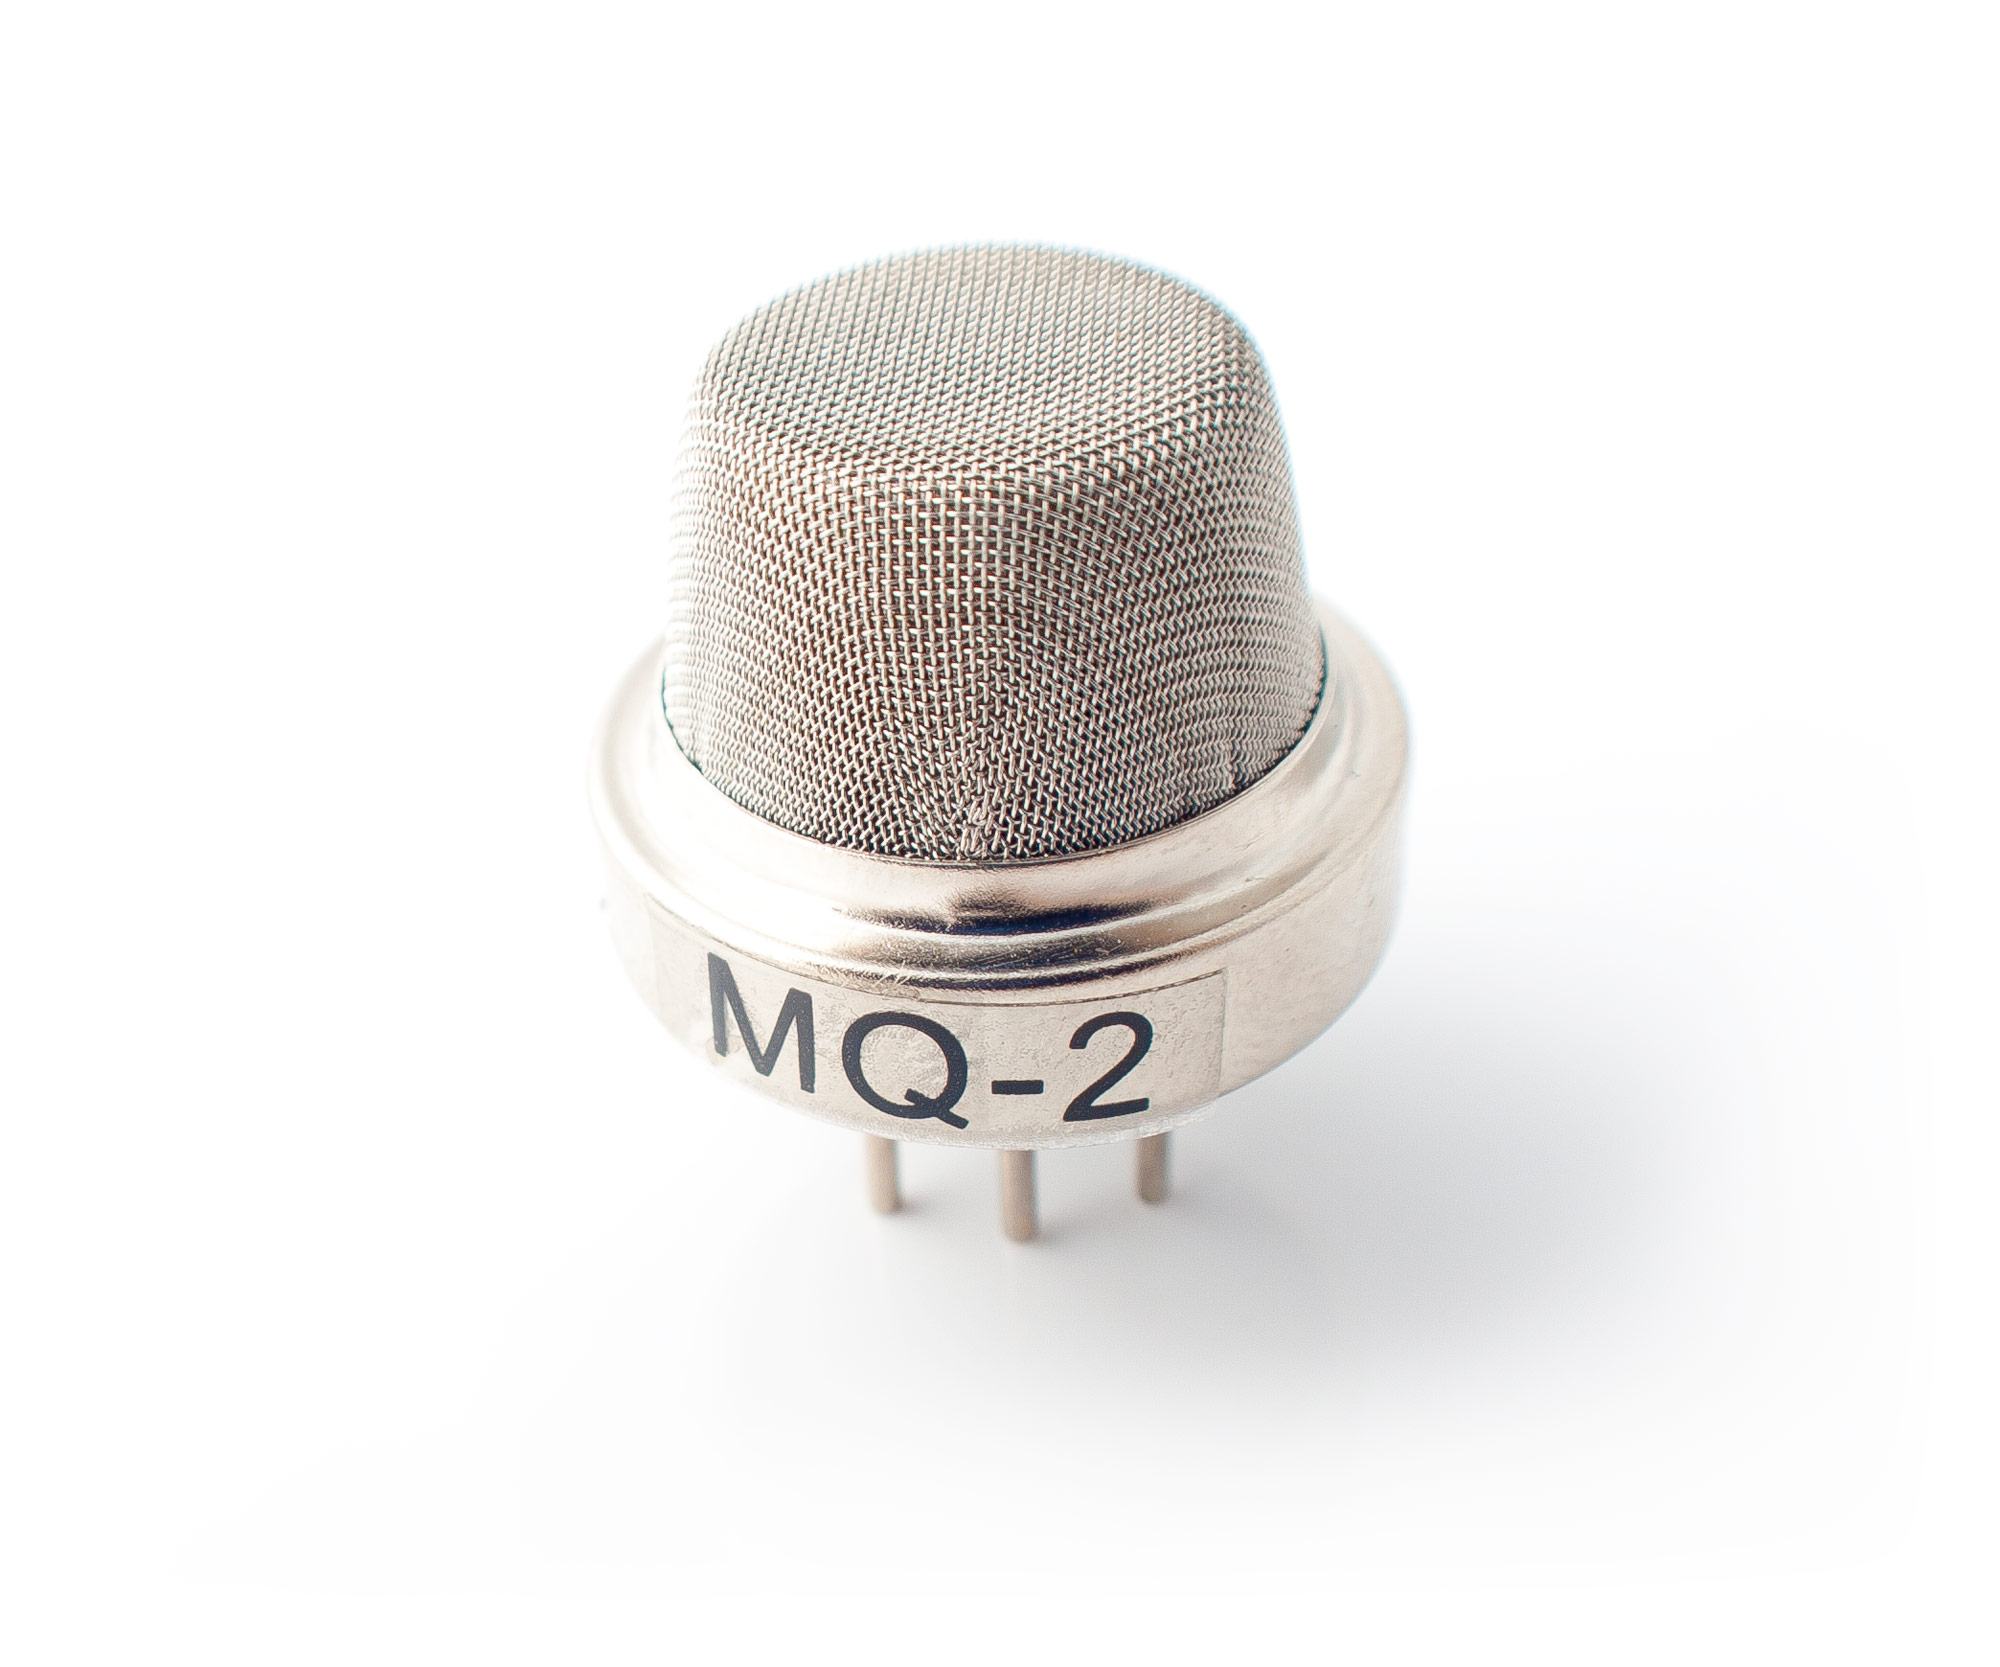
\includegraphics[width=0.5\linewidth]{MQ2}

\subsection{Sensor MH-Z19 NDIR CO2}
MH-Z19 NDIR infrared gas module is a common type, small size sensor, using non-dispersive
infrared (NDIR) principle to detect the existence of CO 2 in the air, with good selectivity, non-oxygen
dependent and long life. Built-in temperature sensor can do temperature compensation; and it has
digital output and analog voltage output. It is developed by the tight integration of mature infrared absorbing
gas detection technology, precision optical circuit design and superior.

By sending the bytes (0xFF, 0x01, 0x86, 0x00, 0x00, 0x00, 0x00, 0x00, 0x79) to sensor UART it returns
(Starting byte, command, High level, Low level, -, -, -, -, -, checksum).
Then we can calculate: Gas concentration (PPM) = high level * 256 + low level.
The rest is of the return values is not important.
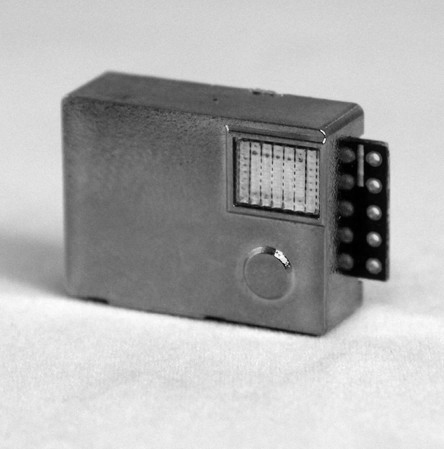
\includegraphics[width=\linewidth]{MH-Z19}


\subsection{Sensor GY-NEO6MV2-GPS}
The NEO-6 module series is a family of stand-alone GPS receivers featuring the high performance u-blox 6
positioning engine. These flexible and cost effective receivers offer numerous connectivity options in a miniature
16 x 12.2 x 2.4 mm package. Their compact architecture and power and memory options make NEO-6 modules
ideal for battery operated mobile devices with very strict cost and space constraints.
The 50-channel u-blox 6 positioning engine boasts a Time-To-First-Fix (TTFF) of under 1 second. The dedicated
acquisition engine, with 2 million correlators, is capable of massive parallel time/frequency space searches,
enabling it to find satellites instantly. Innovative design and technology suppresses jamming sources and
mitigates multipath effects, giving NEO-6 GPS receivers excellent navigation performance even in the most
challenging environments.
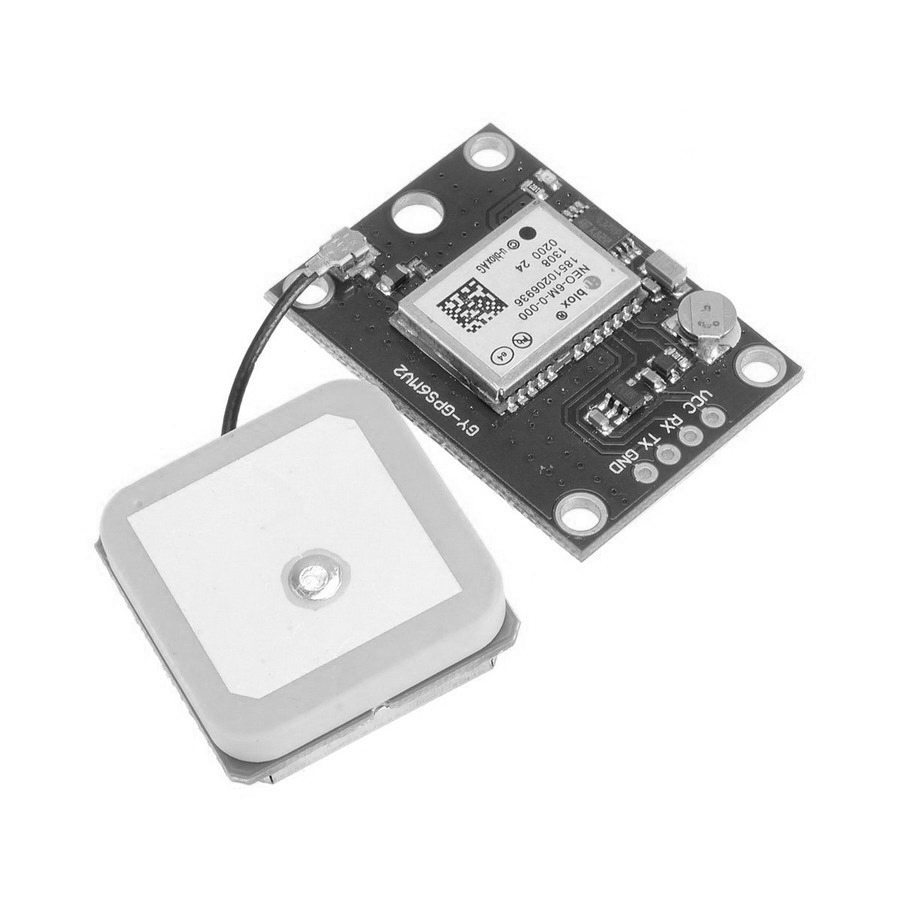
\includegraphics[width=0.5\linewidth]{GY-NEO6MV2-GPS}
